\section{Terrain Modeling from Feature Primitives}
In \cite{CGF:CGF12530} a practical approach is described to model terrains using a construction tree, whos leave nodes are feature primitives. Such primitives describe landmark features, like rivers, mountains, valleys, lakes, and more universal features, like valleys, roughness, hills. The construction tree combines these primitives using a set of operators, which describe the type of combination. 

\subsection{Primitives}
A primitive can either be image based, or skeletal-based. Both primitives feature an elevation function and a weight function that describe the height of the terrain, as well as the potential interaction with other primitives. Skeletal-based primitives profit from a short render time and smaller memory footprint, whereas image-based primitives havea higher memory cost, but provide an easier way to integrate real data into the scene. 

\subsubsection{Skeletal primitives}
Skeletal primitives are defined by a geometric sceleton(point, segment, curve or contour) and a set of parameters that describe the elevation and the weight function. 

A \textbf{disc primitive} contains several parameters, such as the center c and radius r, describing the area of influence, as well as a noise function $\eta(p) $, which controls the local ground roughness. $\{a_i\}$ is a set of decreasing amplitudes, $\{s_i\}$ a set of increasing frequencies. Combining these parameter one can obtain the elevation function
\begin{center}
$ f(p) = c_{z} +  \sum\limits_{i = 0}^{n-1}(a_i\eta((p-c)s_i))$. 
\end{center}

\begin{figure}[htb]
	\centering
	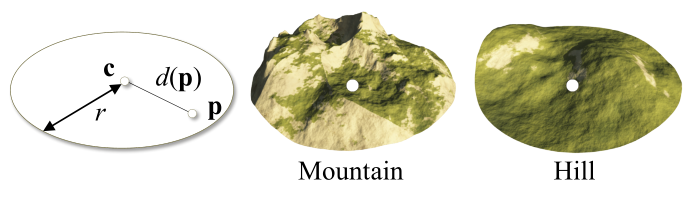
\includegraphics[width=.8\linewidth]{CGFCGF12530/disc_primitive}
	\caption{This figure shows a disc primitive creating a circular landform. The mountain is obtained using ridge-multifractal noise function, smooth hills are created using a turbulence function.}
	\label{fig:disc_primitive}
\end{figure}

\textbf{Curve primitives} are made up of a piecewise curve skelekton $\Gamma$ and a set of profiles $\{c_i\}$. A profile describes a cross section perpendicular to the sceleton. Any function can be used to describe the cross section, in this example each cross section described as a one-dimensional quadratic function. The position is then constructed by interpolation using the curvilinear coordinates. 

One large use of curve primitives is rivers. A river follows its path, described with the curve skeleton. Using different profiles a homogenous shore can be obtained. More complex profiles can describe more larger river systems like deltas and side streams. 
Modifiying the profile accordingly, one can simulate roads with this model, by parametrising the cross section with the road width and defining the elevation of the road in order to allow combination with other primitves in the terrain.

\begin{figure}[htb]
	\centering
	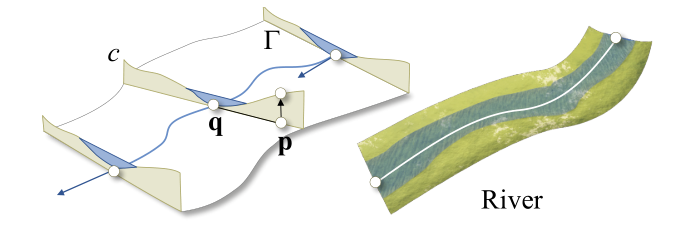
\includegraphics[width=.8\linewidth]{CGFCGF12530/curve_primitive}
	\caption{A curve primitive is used to create a river. $q$ corresponds to the projection of p onto the skeleton.}
	\label{fig:curve_primitive}
\end{figure}

\textbf{Contour primitives} describes a closed curve around a center point and a set of profile curves $\{ c_i \}$. Much like with curve primitives the profile curves discribe the elevation in radial direction. This approach allows to compose more complex features.

\begin{figure}[htb]
	\centering
	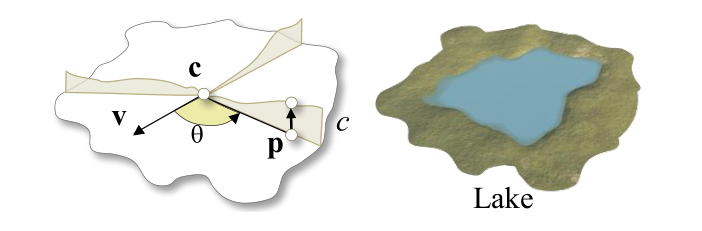
\includegraphics[width=.8\linewidth]{CGFCGF12530/contour_primitive}
	\caption{A contour polygon describes a complex system of polygons. In this figure it is used to describe a lake.}
	\label{fig:contour_primitive}
\end{figure}

\subsubsection{Image primitives}
Complex terrain features are difficult to create procedurally. To add complex feature, such as detailed river shores or sand ripples, image based primitives are used. This process is similar to using a heightfield on a terrain. 

\begin{figure}[htb]
	\centering
	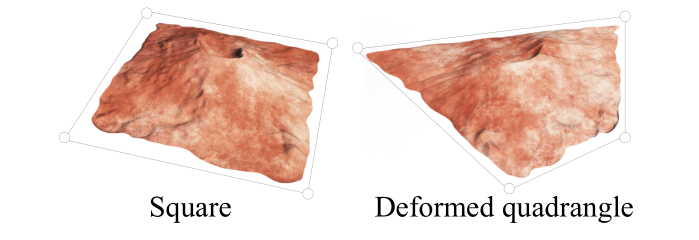
\includegraphics[width=.8\linewidth]{CGFCGF12530/image_primitive}
	\caption{Real data is mapped onto a quadrangle that can be deformed arbitrarily.}
	\label{fig:image_primitive}
\end{figure}


\subsection{Operators}
Much like in Constructive Solid Geometry the inner nodes of the construction tree are operators. These operators combine the elevation function $f$ and weight function $\alpha$ of their sub-trees. For simplicity we consider binary nodes and denote the two sub-trees $A$ and $B$. 

\subsubsection{Blending}
The elevation of two nodes are mixed according to their corresponding weight function. This allows to combine large scale terrain primitives in an effective matter. If two primitives are far away, the do not influence each other. The resulting terrain is the union of to sub-trees. If their regions of interest intersect they blend together.
\begin{figure}[htb]
	\centering
	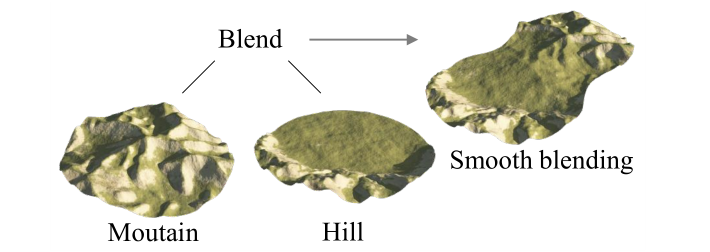
\includegraphics[width=.8\linewidth]{CGFCGF12530/blend_operator}
	\caption{This figure shows a blending of a mountain and hill to a smoother landscape. the areas of interest intersect partly. }
	\label{fig:blend_operator}
\end{figure}
\subsubsection{Replacement}
This operator defines specific local changes in the terrain. Such changes for example are lakes, rivers, roads. If the areas of interest intersect, the elevation in A is replaced with the value in B. 
\begin{figure}[htb]
	\centering
	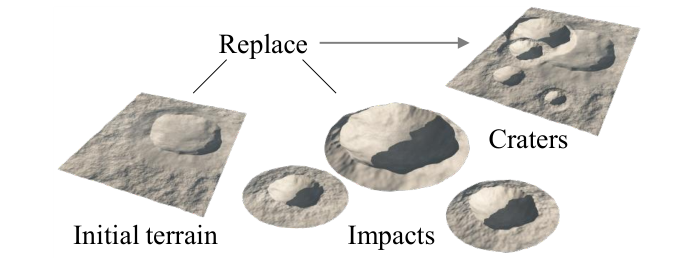
\includegraphics[width=.8\linewidth]{CGFCGF12530/replace_operator}
	\caption{Replacement is used to construct a lunar landscape..}
	\label{fig:replace_operator}
\end{figure}
\subsubsection{Addition}
The addition operator is used to add variations and details to the terrain. The additional elevation to $f_A$ is controlled by the product of $f_B$ and $\alpha_B$
\begin{figure}[htb]
	\centering
	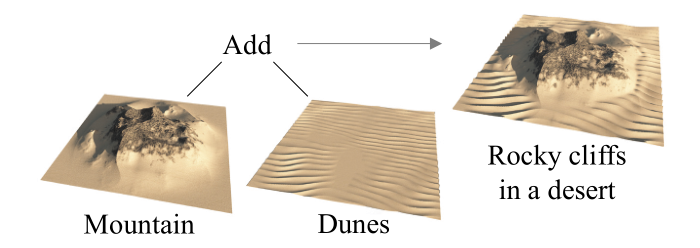
\includegraphics[width=.8\linewidth]{CGFCGF12530/addition_operator}
	\caption{Real data is mapped onto a quadrangle that can be deformed arbitrarily.}
	\label{fig:addition_operator}
\end{figure}
\subsubsection{Warping}
The warping operator allows to distore the shapeoif a surface by displacing the elevation and weight with a certain value, obtained by the warping function. Unlike the other operators, this operator only works on one sub-tree. 
Applying a warp operator to a sub-tree can mask visual artifacts due to repetitive usage of primitives. 
\begin{figure}[htb]
	\centering
	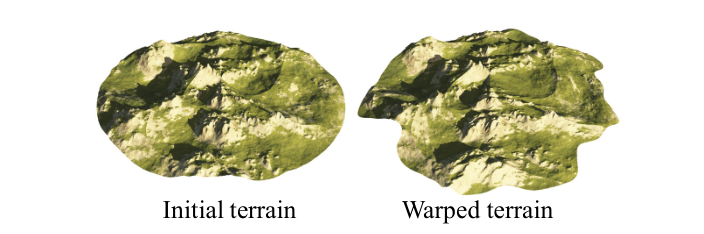
\includegraphics[width=.8\linewidth]{CGFCGF12530/warp_operator}
	\caption{This figure shows a deformed terrain using the warping operator.}
	\label{fig:warp_operator}
\end{figure}
\subsection{Rendering}